% Distributed System project report
\documentclass[11pt, a4paper, twoside, notitlepage]{report}
\usepackage[italian]{babel} %capitolo, sommario e altro in italiano
\usepackage[Lenny]{fncychap} 
\usepackage{fullpage}
\usepackage{setspace}
\usepackage{graphicx}
\usepackage{amsfonts}
\usepackage{wrapfig}  
\usepackage[footnotesize,bf]{caption} %dimensione caption
\usepackage{appendix}
\usepackage[utf8x]{inputenc} %caratteri accentati per linux

\linespread{1.5}    %spaziatura linee
 
\begin{document}
% Logo università Catania
\begin{figure}[h] \hspace*{130pt}

\includegraphics[scale=0.25]{img/unict-bianco.png}
\end{figure}
\begin{center}
\begin{Large}
Università degli Studi di Catania
\end{Large}
\begin{large}
\\Corso di Laurea Magistrale in Ingegneria Informatica
\end{large}
\vspace{30pt}

\textbf{
\begin{Huge}
ITAco
\end{Huge}
}
\begin{large}
\\Linguaggi e Traduttori
\end{large}
\vspace{30pt}
\\Realizzato da:

\begin{Large}
%\begin{flushright}
Alessandro Gallotta, Luca Marturana, Rosario Villari
%\end{flushright}
\end{Large}
\end{center}
\vspace{30pt}
\begin{center}
Docente
\begin{Large}
\\Prof.ssa V. Carchiolo
\end{Large}

\vspace{20pt}
\vfill
\begin{small}
18 Marzo 2012
\end{small}
\end{center}

\thispagestyle{empty} %togli numerazione pagina
\clearpage
\begin{figure}[h] \hspace*{140pt}

\includegraphics[scale=0.5]{img/itaco_logo.png}
\end{figure}
\begin{abstract}
Questo documento riassume brevemente le peculiarità principali del progetto
ITAco da un punto di vista interessato alla dimostrazione ai fini accademici
delle competenze acquisite dagli autori dello stesso nell'ambito della creazione
di linguaggi e compilatori.
\\Il nome è stato scelto seguendo l'idea iniziale di creare un linguaggio di
programmazione molto semplice e intuitivo in lingua italiana, affinché possa
essere facile da utilizzare e didatticamente proficuo per delle categorie di
utenti che possono incontrare difficoltà nella memorizzazione di parole chiave
in lingua straniera.
\\Con lo scopo di perseguire questo obiettivo sono state prese decisioni quali
l'inversione del normale assegnamento dei valori\footnote{L'assegnazione in
ITAco avviene con l'espressione nella parte sinistra e la variabile che riceve
il valore nella parte destra}, che, sebbene risulti a un primo impatto
sconveniente a un utente abituato ad altri linguaggio di programmazione, è
tuttavia molto più intuitivo per un utente abituato ad utilizzare la logica
\emph{della calcolatrice} dove prima si inseriscono i valori e
successivamente li si assegna a una varabile.
\\Altre caratteristiche con questo obiettivo possono essere lette nella sezione
riguardante la sitnassi\footnote{~\ref{sintassi}}. Nell'ambito della facilità di
utilizzo rientrano le scelte di una intuitiva interfaccia grafica mentre,
nell'ambito didattico, la possibilità di traduttre il programma scritto in
diversi linguaggi\footnote{al momento i linguaggi utilizzati sono Ruby, C e
codice Jasmin}.
Questi argomenti sono descritti rispettivamente nella sezione ~\ref{gui} e al capitolo ~\ref{back_end}.
\\Viene inoltre descritto anche l'utilizzo gli strumenti, sia teorici che
pratici, utilizzati per la realizzazione del progetto quali JFlex, CUP, le produzioni
della grammatica utilizzata, i test automatici.

\begin{flushright}
{\bf Keywords:} Compilatori, Cup, JFlex
\end{flushright}
\end{abstract}

\onehalfspacing

%Inizia il conteggio pagine e stampa table of contents (indice)
\setcounter{page}{1}
\setcounter{tocdepth}{3}%profondità table of contents
\tableofcontents

\chapter{Front End}

\section{Scanner}
\subsection{Token utilizzati} 
\section{Parser}
\subsection{Produzioni utilizzate}

\chapter{Back End}
\label{back_end}
\section{Linguaggio target Jasmin}
\section{Linguaggio target C}
\section{Linguaggio target Ruby}

\chapter{Caratteristiche del Linguaggio}
Il lingugaggio, come dalle specifiche richieste, ha le seguenti caratteristiche:
\begin{itemize}
  \item Tipi di dato interi;
  \item Tipi di dato vettore di interi;
  \item Istruzione di assegnazione;
  \item Supporta la definizione e l'invocazione di funzioni i cui argomenti
  possono essere sia interi che vettori di interi e il valore di ritorno è
  rappresentato da un intero;
  \item Possibililtà di controllare il flusso di esecuzione del programma
  attraverso cicli, istruzioni di controllo logiche e il concetto di blocco di
  codice per modellare la sequenza;
  \item Funzionalità di input e output da tastiera.
\end{itemize}

Oltre alle specifiche richieste, sono state aggiunte le seguenti funzionalità
per completezza e per garantire il corretto funzionamento delle specifiche di
cui sopra:
\begin{itemize}
  \item Introduzione degli operatori logici di uguaglianza, maggioranza e
  minoranza;
  \item Gestione parziale dei tipi di dato vero/falso, non gestibili
  direttamente dal programmatore ma attraverso gli operatori logici di
  uguaglianza, maggioranza e minoranza;
  \item Gestione completa degli operatori elementari di somma, sottrazione,
  prodotto e divisione per i tipi di dato interi e gli elementi dei vettori di
  interi.
\end{itemize}
I file sorgente del linguaggi ITAco devono essere salvati in file con estensione
.ita e possono essere creati e modificati con un qualunque editor di testo o
tramite la \emph{Graphic User Interface} descritta alla sezione ~\ref{gui}.
\section{Sintassi Utilizzata}
\label{sintassi}
\subsection{Sintassi nelle funzioni}
La sintassi utilizzata cerca di venire incontro alle utenze non esperte nella
programmazione. Come detto in precedenza, l'assegnazione con la variabile che
riceverà il valore sulla destra è uno di questi accorgimenti.
\\Un altro accorgimento è la definizione delle funzioni nella forma:


\begin{verbatim}
          funzione nome_funzione (arg1 | arg2 | arg3) -> valore_di_ritorno:
                   codice eseguito dalla funzione
          .
\end{verbatim}

o, nel caso in cui non ci sia valore di ritorno:

\begin{verbatim}
          funzione nome_funzione (arg1 | arg2 | arg3):
                   codice eseguito dalla funzione
          .
\end{verbatim}


che richiama la definizione matematica
\[ f(x,y): Dominio \quad -> Codominio\]

La scelta di questa forma per la definizione di funzione risiede anche nel fatto
che la variabile di ritorno, nel caso la funzione ne ritorni uno, è comodamente
accessibile avendola definita direttamente nella firma della funzione.
\\Un altro accorgimento è presente nel caso la funzione abbia come argomento un
vettore. In questo caso, l'argomento sarà definito nella firma della funzione
nella forma:

\begin{verbatim}
          funzione nome_funzione(vettore array[dim]:
                   codice eseguito dalla funzione
          .
\end{verbatim}

in questo modo la dimensione del vettore, anziché essere passata come
altra variabile a parte, è memorizzata nella variabile \emph{dim} racchiuda tra
le parentesi quadre e facilmente riconosciuta come dimensione dell'array.
\\Per assegnare il valore di ritorno di una funzione, la sintassi è:
\begin{verbatim}
          nome_funzione (arg1 | arg2 | arg3) -> variabile_ricevente
\end{verbatim}
nel caso sia necessario far ritornare un intero vettore, è possibile passare
quest'ultimo alla funzione come argomento.
\subsection{Sintassi nelle istruzioni}
Nel resto del codice sorgente, comprese le istruzioni eseguite dalle funzioni,
le seguenti convenzioni sono state adottate:
\begin{itemize}
  \item la virgola rappresenta una terminazione debole, ad esempio la fine di
  una istruzione;
  \item il punto rappresenta una terminazione forte, quale la fine del programma
  o la terminazione di un blocco di codice;
  \item il punto e virgola rappresenta la terminazione del primo blocco nel caso
  della struttura 'se\ldots altrimenti\ldots' :
\end{itemize}
 \begin{verbatim}
          se condizione :
              codice se
          ;
          altrimenti:
              codice altrimenti
          .
 \end{verbatim}
 \begin{itemize}
  \item la concatenzione degli argomenti nell'invocazione o nella definizione
  di una funzione è effettuata tramite il carattere \emph{pipe} '\verb | ' ;
  \item l'istruzione di assegnamento è generata dai caratteri
  '-\verb > ' che simboleggiano una freccia e indicano
  l'assegnazione del valore risultante dall'espressione a sinistra della freccia nella variabile indicata a destra;
  \item le istruzioni di controllo di una condizione e ciclo sono state indicate
  rispettivamente con le parole chiave 'se' e 'finche' e sono necessariamente
  seguite da un blocco di istruzioni;
  \item gli operatori matematici di somma, prodotto, sottrazione e divisione e
  quelli logici di maggioranza e minoranza sono espressi tramite i tradizionali
  simboli. L'unica eccezione è rappresentata dall'uguaglianza:
\end{itemize}
\begin{center}
  \begin{tabular}{ | l | c | }
    \hline
    Somma & +  \\ \hline
    Prodotto & *  \\ \hline
    Sottrazione & -  \\\hline
    Divisione & /  \\ \hline
    Maggioranza & \verb > \\ \hline
    Minoranza & \verb < \\\hline
    Uguaglianza & =  \\\hline
  \end{tabular}
\end{center}
\begin{itemize}
  \item la definizione di una variabile è del tipo:
\end{itemize}
 \begin{verbatim}
          intero nome_variabile,
          vettore nome_vettore[dimensione_vettore]
 \end{verbatim}
 o, nel caso si assegni al volo un valore a una variabile\footnote{nel caso di
 nessun assegnamento, il valore di default è 0}:
 
 \begin{verbatim}
          valore_assegnato -> intero nome_variabile
\end{verbatim}

\begin{itemize}
 \item per la lettura da tastiera di un intero:
\begin{verbatim}
          leggi nome_variabile_ricevente
\end{verbatim}
\item infine, per la scrittura di un intero:
\begin{verbatim}
          scrivi variabile_da_scrivere
\end{verbatim}
mentre, per la scrittura di una stringa:
\begin{verbatim}
          leggi "stringa da scrivere"
\end{verbatim}
\end{itemize} 
\chapter{Altri Strumenti}
In questo capitolo sono elencati degli strumenti che gli autori del progetto
hanno ritenuto opportuno aggiungere per aumentare vuoi l'usabilità e in generale
la qualità del programma finito vuoi la facilità di sviluppo e il bug-tracking.
\section{Test Automatici}
Al fine di velocizzare lo sviluppo e mantenere un alto livello di controllo sui
bug, sono stati introdotti dei test automatici che coprono la gamma di
funzionalità offerte dal linguaggio ITAco. Poiché le specifiche del progetto
richiedevano principalemente la compilazione usando come linguaggio target
\emph{Jasmin}, i test sono stati creati ad hoc per tale linguaggio. La natura di
alto livello degli altri linguaggi target non hanno fatto ritenere al team di
autori che la necessità di creare appositi test superasse il valore del tempo
necessario per crearli.
\\I test funzionano nel seguente modo:
\begin{enumerate}
  \item La classe \emph{JasminTest} compila e carica dei file .ita creati
  appositamente per i test;
  \item la suddetta classe invia determinati valori di input dei quali conosce
  già i risultati;
  \item infine preleva e confronta i risultati ottenuti dal file compilato con
  quelli attesi.
\end{enumerate}
I file di test .ita sono stati creati anche con lo scopo di fornire una suite di
esempi per rendere più facile l'apprendimento della sintassi e delle
funzionalità del linguaggio.
\\Questi esempi mostrano l'utilizzo di svariati strumenti che vanno dal semplice
calcolo e uso dello standard input/output all'utilizzo di funzioni, ricorsione e
semplici algoritmi quali il bubble sort.

\section{Interfaccia}
\label{gui}
La compilazione dei file .ita può avvenire tramite due diversi strumenti
indipendenti che contrappongono a facilità e intuitività di utilizzo una
maggiore portabilità. Essi sono descritti nel seguito di questo capitolo.
\subsection{Graphic User Interface}
La \emph{Graphic User Interface}\footnote{in seguito abbreviata in \emph{GUI}} è
la classica interfaccia grafica gestita con una finestra. Questa \emph{GUI}
fornisce, oltre a degli immediati comandi di compilazione e traduzione del
codice, dei basilari elementi di editor di testo quali la gestione dei file e
la possibilità di modificare il codice sorgente .ita.
\\La portabilità di questa interfaccia è limitata dal tipo di prompt o shell
utilizzato. Infatti, per l'esecuzione immediata del programma generato, è
necessaria una prompt dei comandi nei sistemi \emph{Windows} o un
\emph{gnome-terminal} nei sistemi \emph{Linux}.
L'interfaccia grafica contiene anche una breve guida alla sintassi del
linguaggio accessibile tramite il menù \emph{Aiuto} e un'area di log dove tutto
il log della compilazione è indirizzato.

\begin{figure}[h] \hspace*{30pt} 
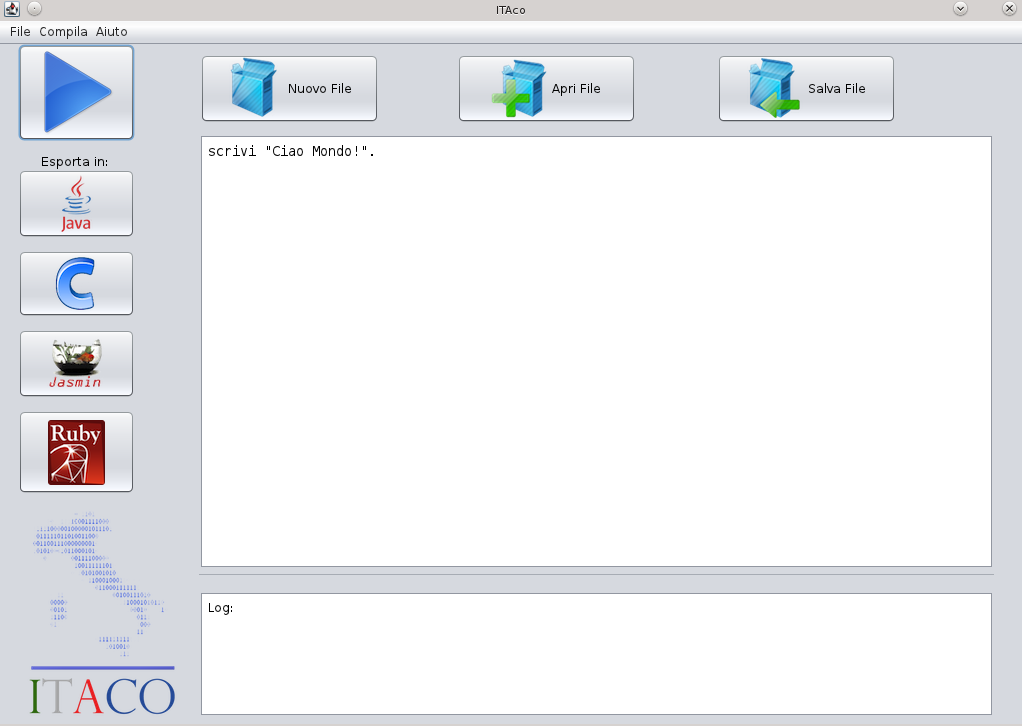
\includegraphics[scale=0.5]{img/gui_itaco.png}
\caption{Finestra principale della GUI}
\end{figure}

\subsection{Command Line Interface}
Oltre all'interfaccia grafica è stato ritenuto importante non tralasciare un
tool da riga di comando\footnote{in seguito ci si riferirà a tale strumento
con \emph{CLI}} che, sebbene possa essere meno intuitivo per il target di utenza
con poca dimestichezza all'utilizzo dei calcolatori, ridimensiona notevolmente
il problema di portabilità della \emph{GUI}, essendo la \emph{CLI} utilizzabile
in ogni sistema su cui sia presente l'ambiene Java.
\\La sintassi per l'utilizzo è
\begin{verbatim}

\end{verbatim}
La \emph{CLI} quindi aggiunge maggiore portabilità e la possibilità di essere
inserita in script.

\end{document}
